% !Mode:: "TeX:UTF-8"
\chapter{后端2}
\begin{mdframed}  
	\textbf{主要目标}
	\begin{enumerate}[labelindent=0em,leftmargin=1.5em]
		\item 理解Pose Graph优化。
		\item 理解因子图优化。
		\item 理解增量式图优化的工作原理。
		\item 通过实验掌握g2o的Pose Graph优化与gtsam的因子图优化。
	\end{enumerate}
\end{mdframed}

上一讲我们重点介绍了以BA为主的图优化。BA能精确地优化每个相机位姿与特征点位置。不过在更大的场景中,大量特征点的存在会严重降低计算效率,导致计算量越来越大以至于无法实时化。本讲介绍两种在更大场景下使用的后端优化方法:位姿图和因子图。

\newpage
\section{位姿图(Pose Graph)}
\subsection{Pose Graph的意义}
带有相机位姿和空间点的图优化称为BA,能够有效地求解大规模的定位与建图问题。但是,随着时间的流逝,机器人的运动轨迹将越来越长,地图规模也将不断增长。像BA这样的方法,计算效率会(令人担忧地)不断下降。根据前面的讨论,我们发现特征点在优化问题中占据了绝大部分。而实际上,经过若干次观测之后,那些收敛的特征点,空间位置估计会收敛至一个值保持不动,而发散的外点则通常看不到了。对收敛点再进行优化,似乎是有些费力不讨好的。因此,我们更倾向于在优化几次之后就把特征点固定住,只把它们看作位姿估计的约束,而不再实际地优化它们的位置估计。

沿着这个思路往下走,我们会想到:是否能够完全不管路标而只管轨迹呢?我们完全可以构建一个只有轨迹的图优化,而位姿节点之间的边,可以由两个关键帧之间通过特征匹配之后得到的运动估计来给定初始值。不同的是,一旦初始估计完成,我们就不再优化那些路标点的位置,而只关心所有的相机位姿之间的联系了。通过这种方式,我们省去了大量的特征点优化的计算,只保留了关键帧的轨迹,从而构建了所谓的位姿图(Pose Graph),如\autoref{fig:pose-graph}~所示。

\begin{figure}[!ht]
	\centering
	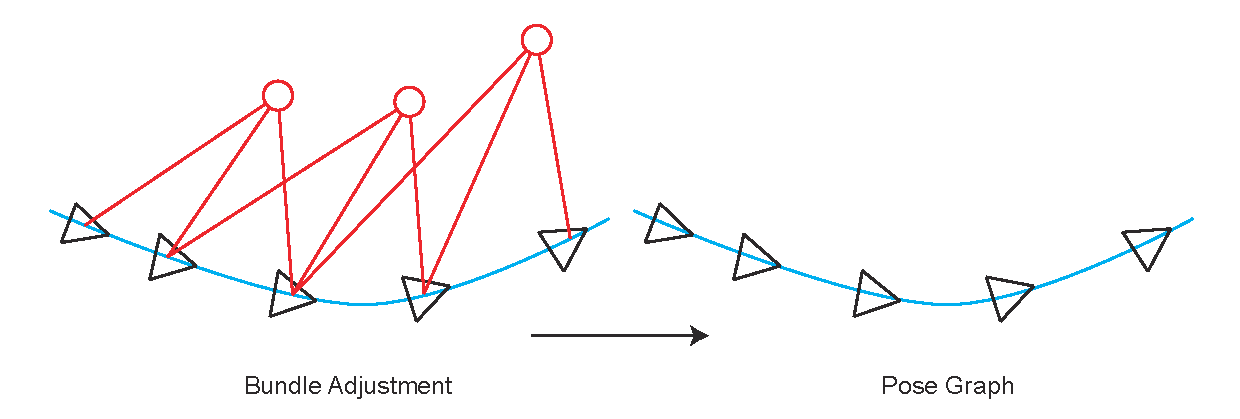
\includegraphics[width=0.8\textwidth]{backend2/posegraph.pdf}
	\caption{Pose Graph示意图。当我们不再优化Bundle Adjustment中的路标点,仅把它们看成对姿态节点的约束时,就得到了一个计算规模减小很多的Pose Graph。}
	\label{fig:pose-graph}
\end{figure}

我们知道,在BA中特征点数量远大于位姿节点。一个关键帧往往关联了数百个关键点,而实时BA的最大计算规模,即使利用稀疏性,在当前的主流CPU上一般也就是几万个点左右。这就限制了SLAM应用场景。所以,当机器人在更大范围的时间和空间中运动时,必须考虑一些解决方式:要么像滑动窗口法那样,丢弃一些历史数据\textsuperscript{\cite{Strasdat2011}};要么像Pose Graph的做法那样,舍弃对路标点的优化,只保留Pose之间的边,使用Pose Graph\textsuperscript{\cite{Dubbelman2015, Lee2014, Latif2013}}。

\clearpage
\subsection{Pose Graph的优化}
那么,Pose Graph图优化中的节点和边都是什么意思呢?这里的节点表示相机位姿,以$\bm{\xi}_1, \cdots, \bm{\xi}_n$来表达。而边,则是两个位姿节点之间相对运动的估计,该估计可能来自于特征点法或直接法,但不管如何,我们估计了,比如说$\bm{\xi}_i$和$\bm{\xi}_j$之间的一个运动$\Delta \bm{\xi}_{ij}$。该运动可以有若干种表达方式,我们取比较自然的一种:
\begin{equation}
\Delta \bm{\xi}_{ij} = \bm{\xi}_i^{-1} \circ \bm{\xi}_j = \ln \left(\exp \left( (-\bm{\xi}_{i})^\wedge \right) \exp \left( \bm{\xi}_j^\wedge \right) \right)^\vee,
\end{equation}
或按李群的写法:
\begin{equation}
\bm{T}_{ij} =\bm{T}_i^{-1} \bm{T}_j.
\end{equation}

按照图优化的思路来看,实际当中该等式不会精确地成立,因此我们设立最小二乘误差,然后和以往一样,讨论误差关于优化变量的导数。这里,我们把上式的$\bm{T}_{ij}$移至等式右侧,构建误差$\bm{e}_{ij}$:
\begin{equation}
\begin{aligned}
\bm{e}_{ij} &= \ln \left( \bm{T}_{ij}^{-1} \bm{T}_i^{-1} \bm{T}_j \right)^\vee \\ 
&= \ln \left( \exp((-\bm{\xi}_{ij})^\wedge) \exp( (-\bm{\xi}_i)^\wedge) \exp(\bm{\xi}_j^{\wedge} ) \right)^\vee.
\end{aligned}
\end{equation}

注意优化变量有两个:$\bm{\xi}_i$和$\bm{\xi}_j$,因此我们求$\bm{e}_{ij}$关于这两个变量的导数。按照李代数的求导方式,给$\bm{\xi}_i$和$\bm{\xi}_j$各一个左扰动:$ \bm{\delta \xi}_i$和$ \bm{\delta \xi}_j$。于是误差变为
\begin{equation}
\hat{ \bm{e}}_{ij} = \ln \left( \bm{T}_{ij}^{-1}  \bm{T}_i^{-1} \exp((-\bm{\delta \xi}_i)^\wedge) \exp(\delta \bm{\xi}_j^\wedge) \bm{T}_j  \right)^\vee.
\end{equation}

该式中,两个扰动项被夹在了中间。为了利用BCH近似,我们希望把扰动项移至式子左侧或右侧。回忆第4讲习题中的伴随性质,即式\eqref{eq:adjSE3}。如果你没有做过这个习题,那就暂时想当然地认为其正确。
\begin{equation}
\exp \left( \left( \mathrm{Ad}(\bm{T}) \bm{\xi} \right) ^\wedge \right) = \bm{T} \exp(\bm{\xi}^\wedge)\bm{T}^{-1}.
\end{equation}

稍加改变,有:
\begin{equation}
\exp(\bm{\xi}^\wedge)\bm{T} = \bm{T} \exp \left( \left( \mathrm{Ad}(\bm{T}^{-1}) \bm{\xi} \right) ^\wedge \right) .
\end{equation}

该式表明,通过引入一个伴随项,我们能够“交换”扰动项左右侧的$\bm{T}$。利用它,可以将扰动挪到最右(当然最左亦可),导出右乘形式的雅可比矩阵(挪到左边时形成左乘):
\clearpage
\begin{equation}
\begin{aligned}
\hat{ \bm{e}}_{ij} &= \ln \left( \bm{T}_{ij}^{-1}  \bm{T}_i^{-1} \exp((-\bm{\delta \xi}_i)^\wedge) \exp(\delta \bm{\xi}_j^\wedge) \bm{T}_j  \right)^\vee\\
&= \ln \left( \bm{T}_{ij}^{-1} \bm{T}_i^{-1} \bm{T}_j \exp \left( \left(- \mathrm{Ad}(\bm{T}_j^{-1}) \bm{\delta \xi}_i \right)^\wedge \right) \exp \left( \left( \mathrm{Ad}(\bm{T}_j^{-1})  \bm{\delta\xi}_j\right)^\wedge \right) \right)^\vee \\ 
&\approx \ln \left( \bm{T}_{ij}^{-1} \bm{T}_i^{-1} \bm{T}_j \left[ \bm{I} - (\mathrm{Ad}(\bm{T}_j^{-1}) \bm{\delta \xi}_i)^\wedge + (\mathrm{Ad}(\bm{T}_j^{-1})  \bm{\delta \xi}_j)^{\wedge} \right] \right)^\vee \\
& \approx \bm{e}_{ij} + \frac{\partial \bm{e}_{ij}}{\partial \bm{\delta \xi}_i} \bm{\delta \xi}_i + \frac{\partial \bm{e}_{ij}}{\partial \bm{\delta \xi}_j} \bm{\delta \xi}_j
\end{aligned}.
\end{equation}

因此,按照李代数上的求导法则,我们求出了误差关于两个位姿的雅可比矩阵。关于$\bm{T}_i$的:
\begin{equation}
\frac{\partial \bm{e}_{ij}}{\partial \bm{\delta \xi}_i} = - \bm{\mathcal{J}}_r^{-1}(\bm{e}_{ij}) \mathrm{Ad}(\bm{T}_j^{-1}).
\end{equation}
以及关于$\bm{T}_j$的:
\begin{equation}
\frac{\partial \bm{e}_{ij}}{\partial \bm{\delta \xi}_j} = \bm{\mathcal{J}}_r^{-1}(\bm{e}_{ij}) \mathrm{Ad}(\bm{T}_j^{-1}).
\end{equation}

如果读者觉得这部分求导理解起来有困难,可以回到第4讲温习一下李代数部分的内容。不过,前面也说过,由于$\mathfrak{se}(3)$上的左右雅可比$\bm{\mathcal{J}}_r$形式过于复杂,我们通常取它们的近似。如果误差接近于零,我们就可以设它们近似为$\bm{I}$或
\begin{equation}
\bm{\mathcal{J}}_r^{-1}(\bm{e}_{ij}) \approx \bm{I} + \frac{1}{2} 
\left[ 
{\begin{array}{*{20}{c}}
	{{\bm{\phi}_{\bm{e}} ^ \wedge }}&{{\bm{\rho}_{\bm{e}} ^ \wedge }}\\
	{\bm{0}}&{{\bm{\phi}_{\bm{e}} ^ \wedge }}
\end{array}} 
\right].
\end{equation}

理论上讲,即使在优化之后,由于每条边给定的观测数据并不一致,误差通常也不见得近似于零,所以简单地把这里的$\bm{\mathcal{J}}_r$设置为$\bm{I}$会有一定的损失。稍后我们将通过实践来看看理论上的区别是否明显。

了解雅可比求导后,剩下的部分就和普通的图优化一样了。简而言之,所有的位姿顶点和位姿——位姿边构成了一个图优化,本质上是一个最小二乘问题,优化变量为各个顶点的位姿,边来自于位姿观测约束。记$\mathcal{E}$为所有边的集合,那么总体目标函数为
\begin{equation}
\mathop {\min }\limits_{\bm{\xi}} \frac{1}{2}\sum\limits_{i,j \in \mathcal{E}} \bm{e}_{ij}^\mathrm{T} \bm{\Sigma}_{ij}^{-1} \bm{e}_{ij}.
\end{equation}

我们依然可以用高斯牛顿法、列文伯格—马夸尔特方法等求解此问题,除了用李代数表示优化位姿以外,别的都是相似的。根据先前的经验,这自然可以用Ceres或g2o进行求解。我们不再讨论优化的详细过程,上一讲已经讲得够多了。

\section{实践:位姿图优化}
\subsection{g2o原生位姿图}
下面演示使用g2o进行位姿图优化。首先,请读者用g2o\_viewer打开我们预先生成的仿真位姿图,位于slambook/ch11/sphere.g2o中,如\autoref{fig:sphere-before}~所示。

\begin{figure}[!htp]
	\centering
	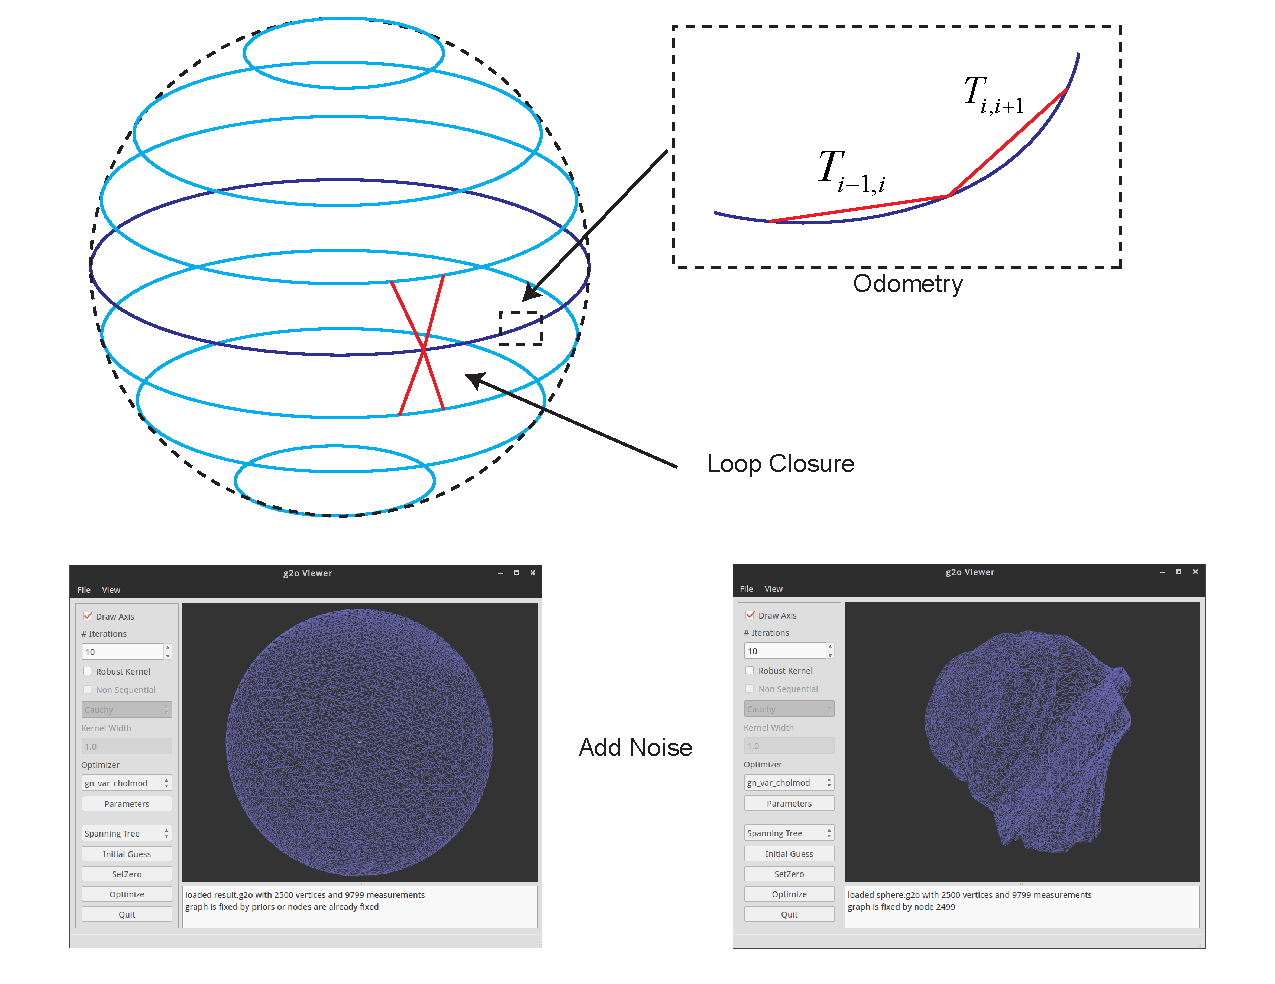
\includegraphics[width=1.0\textwidth]{backend2/sphere-before.pdf}
	\caption{g2o仿真产生的位姿图。真值是完整的球形,在真值上添加噪声后得到带累计误差的仿真数据。}
	\label{fig:sphere-before}
\end{figure}

该位姿图是由g2o自带的create sphere程序仿真生成的。它的真实轨迹为一个球,由从下往上的多个层组成。每层为一个正圆形,很多个大小不一的圆形层组成了一个完整的球体,共包含2500个位姿节点(\autoref{fig:sphere-before}~左上),可以看成一个转圈上升的过程。然后,仿真程序生成了$t-1$到$t$时刻的边,称为odometry边(里程计)。此外,又生成层与层之间的边,称为loop closure(回环,将在下一讲详细介绍)。随后,在每条边上添加观测噪声,并根据里程计边的噪声,重新设置节点的初始值。这样,就得到了带累积误差的位姿图数据(\autoref{fig:sphere-before}~右下)。它局部看起来像球体的一部分,但整体形状与球体相差甚远。现在我们从这些带噪声的边和节点初始值出发,尝试优化整个位姿图,得到近似真值的数据。

当然,实际当中的机器人肯定不会出现这样正球形的运动轨迹,以及如此完整的里程计与回环观测数据。仿真成正球的好处是我们能够直观地看到优化结果是否正确(只要看它各个角度圆不圆就行了)。读者可以单击g2o\_viewer中的optimize函数,看到每步的优化结果和收敛的过程。另一方面,sphere.g2o也是一个文本文件,可以用文本编辑器打开,查看它里面的内容。文件前半部分由节点组成,后半部分则是边:

\begin{lstlisting}
VERTEX_SE3:QUAT 0 -0.125664 -1.53894e-17 99.9999 0.706662 4.32706e-17 0.707551 -4.3325e-17 
......
EDGE_SE3:QUAT 1524 1574 -0.210399 -0.0101193 -6.28806 -0.00122939 0.0375067 -2.85291e-05 0.999296 10000 0 0 0 0 0 10000 0 0 0 0 10000 0 0 0 40000 0 0 40000 0 40000 
\end{lstlisting}

可以看到,节点类型是VERTEX\_SE3,表达一个相机位姿。g2o默认使用四元数和平移向量表达位姿,所以后面的字段意义为:ID,$t_x, t_y, t_z, q_x, q_y, q_z, q_w$。前3个为平移向量元素,后4个为表示旋转的单位四元数。同样,边的信息为两个节点的ID,$t_x, t_y, t_z, q_x, q_y, q_z, q_w$,信息矩阵的右上角(由于信息矩阵为对称阵,只需保存一半即可)。可以看到这里把信息矩阵设成了对角阵。

为了优化该位姿图,我们可以使用g2o默认的顶点和边,它们是由四元数表示的。由于仿真数据也是g2o生成的,所以用g2o本身优化就无须我们多做什么工作了,只需配置一下优化参数即可。程序slambook/ch11/pose\_graph\_g2o\_SE3.cpp演示了如何使用列文伯格—马夸尔特方法对该位姿图进行优化,并把结果存储至result.g2o文件中。

\begin{lstlisting}[language=c++,caption=slambook/ch11/pose\_graph\_g2o\_SE3.cpp]
#include <iostream>
#include <fstream>
#include <string>

#include <g2o/types/slam3d/types_slam3d.h>
#include <g2o/core/block_solver.h>
#include <g2o/core/optimization_algorithm_levenberg.h>
#include <g2o/core/optimization_algorithm_gauss_newton.h>
#include <g2o/solvers/dense/linear_solver_dense.h>
#include <g2o/solvers/cholmod/linear_solver_cholmod.h>
using namespace std;

/************************************************
* 本程序演示如何用 g2o solver 进行位姿图优化
* sphere.g2o 是人工生成的一个 Pose graph ,我们来优化它。
* 尽管可以直接通过 load 函数读取整个图,但我们还是自己来实现读取代码,以期获得更深刻的理解。
* 这里使用 g2o/types/slam3d/ 中的 SE3 表示位姿,它实质上是四元数而非李代数。
* **********************************************/

int main( int argc, char** argv )
{
	if ( argc != 2 )
	{
		cout<<"Usage: pose_graph_g2o_SE3 sphere.g2o"<<endl;
		return 1;
	}
	ifstream fin( argv[1] );
	if ( !fin )
	{
		cout<<"file "<<argv[1]<<" does not exist."<<endl;
		return 1;
	}
	
	typedef g2o::BlockSolver<g2o::BlockSolverTraits<6,6>> Block;  // 6x6 BlockSolver
	Block::LinearSolverType* linearSolver = new g2o::LinearSolverCholmod<Block::PoseMatrixType>();
	Block* solver_ptr = new Block( linearSolver );      // 矩阵块求解器
	g2o::OptimizationAlgorithmLevenberg* solver=new g2o::OptimizationAlgorithmLevenberg(solver_ptr);
	g2o::SparseOptimizer optimizer;     // 图模型
	optimizer.setAlgorithm( solver );   // 设置求解器
	
	int vertexCnt = 0, edgeCnt = 0; // 顶点和边的数量
	while ( !fin.eof() )
	{
		string name;
		fin>>name;
		if ( name == "VERTEX_SE3:QUAT" )
		{
			// SE3 顶点
			g2o::VertexSE3* v = new g2o::VertexSE3();
			int index = 0;
			fin>>index;
			v->setId( index );
			v->read(fin);
			optimizer.addVertex(v);
			vertexCnt++;
			if ( index==0 )
			v->setFixed(true);
		}
		else if ( name=="EDGE_SE3:QUAT" )
		{
			// SE3−SE3 边
			g2o::EdgeSE3* e = new g2o::EdgeSE3();
			int idx1, idx2;     // 关联的两个顶点
			fin>>idx1>>idx2;
			e->setId( edgeCnt++ );
			e->setVertex( 0, optimizer.vertices()[idx1] );
			e->setVertex( 1, optimizer.vertices()[idx2] );
			e->read(fin);
			optimizer.addEdge(e);
		}
		if ( !fin.good() ) break;
	}
	
	cout<<"read total "<<vertexCnt<<" vertices, "<<edgeCnt<<" edges."<<endl;
	
	cout<<"prepare optimizing ..."<<endl;
	optimizer.setVerbose(true);
	optimizer.initializeOptimization();
	cout<<"calling optimizing ..."<<endl;
	optimizer.optimize(30);
	
	cout<<"saving optimization results ..."<<endl;
	optimizer.save("result.g2o");
	
	return 0;
}
\end{lstlisting}

我们选择了$6\times6$的块求解器,使用列文伯格—马夸尔特下降方式,迭代次数选择30次。调用此程序对位姿图进行优化:
\begin{lstlisting}
$ build/pose_graph_g2o_SE3 sphere.g2o 
read total 2500 vertices, 9799 edges.
prepare optimizing ...
calling optimizing ...
iteration= 0  chi2= 1023011093.967638 time= 0.851879 cumTime= 0.851879 edges= 9799 schur= 0 lambda= 805.622433 levenbergIter= 1
iteration= 1  chi2= 385118688.233188  time= 0.863567 cumTime= 1.71545  edges= 9799 schur= 0 lambda= 537.081622 levenbergIter= 1
iteration= 2  chi2= 166223726.693659  time= 0.861235 cumTime= 2.57668  edges= 9799 schur= 0 lambda= 358.054415 levenbergIter= 1
iteration= 3  chi2= 86610874.269316   time= 0.844105 cumTime= 3.42079  edges= 9799 schur= 0 lambda= 238.702943 levenbergIter= 1
iteration= 4  chi2= 40582782.710190   time= 0.862221 cumTime= 4.28301  edges= 9799 schur= 0 lambda= 159.135295 levenbergIter= 1
......
iteration= 28 chi2= 45095.174398 time= 0.869451 cumTime= 30.0809 edges= 9799 schur= 0 lambda= 0.003127 levenbergIter= 1
iteration= 29 chi2= 44811.248504 time= 1.76326  cumTime= 31.8442 edges= 9799 schur= 0 lambda= 0.003785 levenbergIter= 2
saving optimization results ...
\end{lstlisting}

然后,用g2o\_viewer打开result.g2o查看结果,如\autoref{fig:result-SE3}~所示。
\begin{figure}[!ht]
	\centering
	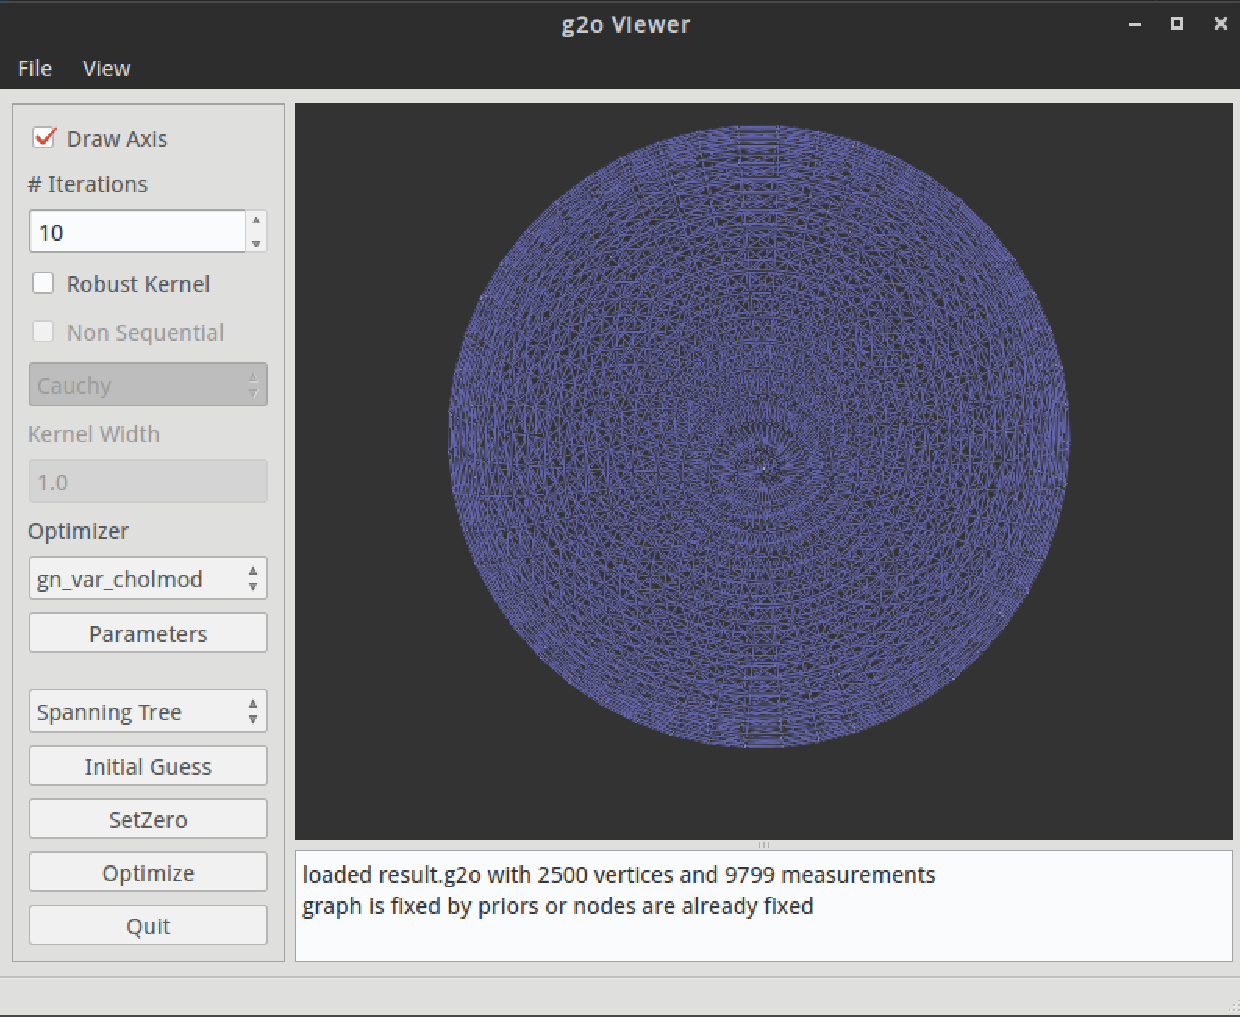
\includegraphics[width=0.75\textwidth]{backend2/result-SE3.pdf}
	\caption{使用g2o自带的顶点与边求解的结果。}
	\label{fig:result-SE3}
\end{figure}

结果从一个不规则的形状优化成了一个看起来完整的球。这个过程实质上和我们单击g2o\_viewer上的Optimize按钮没有区别。下面,我们根据前面的李代数推导来实现一下李代数上的优化。

\subsection{李代数上的位姿图优化}
还记得我们用Sophus来表达李代数的事情吗?我们来试试把Sophus用到g2o中定义自己的顶点和边吧。

\clearpage
\begin{lstlisting}[language=c++,caption=slambook/ch11/pose\_graph\_g2o\_lie\_algebra.cpp(片段)]
#include <iostream>
#include <fstream>
#include <string>
#include <Eigen/Core>

#include <g2o/core/base_vertex.h>
#include <g2o/core/base_binary_edge.h>
#include <g2o/core/block_solver.h>
#include <g2o/core/optimization_algorithm_levenberg.h>
#include <g2o/core/optimization_algorithm_gauss_newton.h>
#include <g2o/core/optimization_algorithm_dogleg.h>
#include <g2o/solvers/dense/linear_solver_dense.h>
#include <g2o/solvers/cholmod/linear_solver_cholmod.h>

#include <sophus/se3.h>
#include <sophus/so3.h>
using namespace std;
using Sophus::SE3;
using Sophus::SO3;

/************************************************
* 本程序演示如何用 g2o solver 进行位姿图优化
* sphere.g2o 是人工生成的一个 Pose graph ,我们来优化它。
* 尽管可以直接通过 load 函数读取整个图,但我们还是自己来实现读取代码,以期获得更深刻的理解。
* 本节使用李代数表达位姿图,节点和边的方式为自定义。
* **********************************************/

typedef Eigen::Matrix<double,6,6> Matrix6d;

// 给定误差求 J_R^{-1} 的近似
Matrix6d JRInv( SE3 e )
{
	Matrix6d J;
	J.block(0,0,3,3) = SO3::hat(e.so3().log());
	J.block(0,3,3,3) = SO3::hat(e.translation());
	J.block(3,0,3,3) = Eigen::Matrix3d::Zero(3,3);
	J.block(3,3,3,3) = SO3::hat(e.so3().log());
	J = J*0.5 + Matrix6d::Identity();
	return J;
}
// 李代数顶点
typedef Eigen::Matrix<double, 6, 1> Vector6d;
class VertexSE3LieAlgebra: public g2o::BaseVertex<6, SE3>
{
public:
	EIGEN_MAKE_ALIGNED_OPERATOR_NEW
	bool read ( istream& is )
	{
		double data[7];
		for ( int i=0; i<7; i++ )
		is>>data[i];
		setEstimate ( SE3 (
			Eigen::Quaterniond ( data[6],data[3], data[4], data[5] ),
			Eigen::Vector3d ( data[0], data[1], data[2] )
		));
	}
	
	bool write ( ostream& os ) const
	{
		os<<id()<<" ";
		Eigen::Quaterniond q = _estimate.unit_quaternion();
		os<<_estimate.translation().transpose()<<" ";
		os<<q.coeffs()[0]<<" "<<q.coeffs()[1]<<" "<<q.coeffs()[2]<<" "<<q.coeffs()[3]<<endl;
		return true;
	}
	
	virtual void setToOriginImpl()
	{
		_estimate = Sophus::SE3();
	}
	// 左乘更新
	virtual void oplusImpl ( const double* update )
	{
		Sophus::SE3 up (
			Sophus::SO3 ( update[3], update[4], update[5] ),
			Eigen::Vector3d ( update[0], update[1], update[2] )
		);
		_estimate = up*_estimate;
	}
};

// 两个李代数节点之边
class EdgeSE3LieAlgebra: public g2o::BaseBinaryEdge<6, SE3, VertexSE3LieAlgebra, VertexSE3LieAlgebra>
{
public:
	EIGEN_MAKE_ALIGNED_OPERATOR_NEW
	bool read ( istream& is )
	{
		double data[7];
		for ( int i=0; i<7; i++ )
		is>>data[i];
		Eigen::Quaterniond q ( data[6], data[3], data[4], data[5] );
		q.normalize();
		setMeasurement (
			Sophus::SE3 ( q, Eigen::Vector3d ( data[0], data[1], data[2] ) ) 
		);
		for ( int i=0; i<information().rows() && is.good(); i++ )
			for ( int j=i; j<information().cols() && is.good(); j++ )
			{
				is >> information() ( i,j );
				if ( i!=j )
					information() ( j,i ) =information() ( i,j );
			}
		return true;
	}
	bool write ( ostream& os ) const
	{
		VertexSE3LieAlgebra* v1 = static_cast<VertexSE3LieAlgebra*> (_vertices[0]);
		VertexSE3LieAlgebra* v2 = static_cast<VertexSE3LieAlgebra*> (_vertices[1]);
		os<<v1->id()<<" "<<v2->id()<<" ";
		SE3 m = _measurement;
		Eigen::Quaterniond q = m.unit_quaternion();
		os<<m.translation().transpose()<<" ";
		os<<q.coeffs()[0]<<" "<<q.coeffs()[1]<<" "<<q.coeffs()[2]<<" "<<q.coeffs()[3]<<" ";
		// information matrix 
		for ( int i=0; i<information().rows(); i++ )
			for ( int j=i; j<information().cols(); j++ )
			{
				os << information() ( i,j ) << " ";
			}
		os<<endl;
		return true;
	}
	
	// 误差计算与书中推导一致
	virtual void computeError()
	{
		Sophus::SE3 v1 = (static_cast<VertexSE3LieAlgebra*> (_vertices[0]))->estimate();
		Sophus::SE3 v2 = (static_cast<VertexSE3LieAlgebra*> (_vertices[1]))->estimate();
		_error = (_measurement.inverse()*v1.inverse()*v2).log();
	}
	
	// 雅可比计算
	virtual void linearizeOplus()
	{
		Sophus::SE3 v1 = (static_cast<VertexSE3LieAlgebra*> (_vertices[0]))->estimate();
		Sophus::SE3 v2 = (static_cast<VertexSE3LieAlgebra*> (_vertices[1]))->estimate();
		Matrix6d J = JRInv(SE3::exp(_error));
		// 尝试把J近似为I?
		_jacobianOplusXi = - J* v2.inverse().Adj();
		_jacobianOplusXj = J*v2.inverse().Adj();
	}
};
\end{lstlisting}

为了实现对g2o文件的存储和读取,本节例程实现了read和write函数,并且“伪装”成g2o内置的SE3顶点,使得g2o\_viewer能够认识并渲染它。事实上,除了内部使用Sophus的李代数表示之外,从外部看起来没有什么区别。

值得注意的是这里雅可比的计算过程。我们有若干种选择:一是不提供雅可比计算函数,让g2o自动计算数值雅可比。二是提供完整或近似的雅可比计算过程。这里我们用JRInv()函数提供近似的$\bm{\mathcal{J}}_r^{-1}$。读者可以尝试把它近似为$\bm{I}$,或者干脆注释掉oplusImpl函数,看看结果会有什么区别。

之后调用g2o进行优化问题:

\begin{lstlisting}
$ build/pose_graph_g2o_lie sphere.g2o    
read total 2500 vertices, 9799 edges.
prepare optimizing ...
calling optimizing ...
iteration= 0  chi2= 781963143.389706 time= 1.9322  cumTime= 1.9322  edges= 9799 schur= 0 lambda= 6706.585223 levenbergIter= 1
iteration= 1  chi2= 236521032.458035 time= 1.91309 cumTime= 3.84529 edges= 9799 schur= 0 lambda= 2235.528408 levenbergIter= 1
iteration= 2  chi2= 142934798.398778 time= 1.9792  cumTime= 5.8245  edges= 9799 schur= 0 lambda= 745.176136  levenbergIter= 1
iteration= 3  chi2= 84490229.050137  time= 2.03394 cumTime= 7.85844 edges= 9799 schur= 0 lambda= 248.392045  levenbergIter= 1
iteration= 4  chi2= 42690811.624643  time= 2.05149 cumTime= 9.90993 edges= 9799 schur= 0 lambda= 82.797348   levenbergIter= 1
......
iteration= 21 chi2= 127607.121623    time= 1.9686  cumTime= 43.526  edges= 9799 schur= 0 lambda= 0.000712    levenbergIter= 1
iteration= 22 chi2= 127578.889888    time= 1.94773 cumTime= 45.4737 edges= 9799 schur= 0 lambda= 0.000237    levenbergIter= 1
iteration= 23 chi2= 127578.158794    time= 1.98009 cumTime= 47.4538 edges= 9799 schur= 0 lambda= 0.000079    levenbergIter= 1
iteration= 24 chi2= 127578.157859    time= 2.04546 cumTime= 49.4993 edges= 9799 schur= 0 lambda= 0.000053    levenbergIter= 1
iteration= 25 chi2= 127578.157859    time= 1.96722 cumTime= 51.4665 edges= 9799 schur= 0 lambda= 0.000035    levenbergIter= 1
iteration= 26 chi2= 127578.157859    time= 2.11235 cumTime= 53.5789 edges= 9799 schur= 0 lambda= 0.000023    levenbergIter= 1
iteration= 27 chi2= 127578.157859    time= 3.29151 cumTime= 56.8704 edges= 9799 schur= 0 lambda= 0.000031    levenbergIter= 2
iteration= 28 chi2= 127578.157859    time= 3.20302 cumTime= 60.0734 edges= 9799 schur= 0 lambda= 0.000042    levenbergIter= 2
iteration= 29 chi2= 127578.157859    time= 5.56337 cumTime= 65.6368 edges= 9799 schur= 0 lambda= 0.001779    levenbergIter= 4
saving optimization results ...
\end{lstlisting}

我们发现,迭代23次后,总体误差保持不变,事实上可以让优化算法停止了。而上一个实验中,用满了30次迭代后误差仍在下降\footnote{请注意,尽管数值上看此处的误差要大一些,但是由于我们自定义边时重新定义了误差的计算方式,所以此处数值的大小并不能直接用于比较。}。在调用优化后,查看result\_lie.g2o观察它的结果,如\autoref{fig:result-lie}~所示。从肉眼上看不出任何区别。

\begin{figure}[!ht]
	\centering
	\includegraphics[width=0.72\textwidth]{backend2/result-lie.pdf}
	\caption{使用李代数自定义节点与边优化后的结果。}
	\label{fig:result-lie}
\end{figure}

如果你在这个g2o\_viewer界面按下Optimize按钮,g2o将使用它自带的SE3顶点进行优化,你可以在下方文本框中看到:

\begin{lstlisting}
loaded result_lie.g2o with 2500 vertices and 9799 measurements
graph is fixed by node 2499
# Using CHOLMOD poseDim -1 landMarkDim -1 blockordering 0
Preparing (no marginalization of Landmarks)
iteration= 0 chi2= 44360.509723 time= 0.567504 cumTime= 0.567504 edges= 9799 schur= 0
iteration= 1 chi2= 44360.471110 time= 0.595993 cumTime= 1.1635   edges= 9799 schur= 0
iteration= 2 chi2= 44360.471110 time= 0.582909 cumTime= 1.74641  edges= 9799 schur= 0
\end{lstlisting}

整体误差在SE3边的度量下为44360,略小于之前30次迭代时的44811。这说明使用李代数进行优化后,我们在更少的迭代次数下得到了更好的结果\footnote{由于没有做更多的实验,所以该结论只在“球”这个例子上有效。}。

\subsection{小结}
球的例子是一个比较有代表性的案例。它具有和实际中相似的里程计边(Odometry)和回环边(Loop Closure),这也正是实际SLAM中一个位姿图中可能有的东西。同时,“球”也具有一定的计算规模:它总共有2,500个位姿节点和近10,000条边,我们发现优化它费了不少时间(相对于实时性要求很强的前端来说)。另一方面,一般认为位姿图是结构最简单的图之一。在我们不假设机器人如何运动的前提下,很难再进一步讨论它的稀疏性了——因为机器人可能会直线往前运动,形成带状的位姿图,是稀疏的;也可能是“左手右手一个慢动作”,形成大量的小型回环需要优化(Loopy motion),从而变成像“球”那样比较稠密的位姿图。无论如何,在没有进一步的信息之前,我们似乎无法再利用位姿图的求解结构了。

自PTAM\textsuperscript{\cite{Klein2007}}提出以来,人们就意识到,后端的优化没必要实时地响应前端的图像数据。人们倾向于把前端和后端分开,运行于两个独立线程之中,历史上称为跟踪(Tracking)和建图(Mapping)——虽然如此叫,建图部分主要是指后端的优化内容。通俗地说,前端需要实时响应视频的速度,例如每秒30帧;而优化可以慢悠悠地运行,只要在优化完成时把结果返回给前端即可。所以我们通常不会对后端优化提出很高的速度要求。

\section{\textsuperscript{\ttfamily *}因子图优化初步}
\subsection{贝叶斯网络}
下面,我们从另一个角度来看后端优化:所谓的因子图(Factor Graph)优化。由于这部分内容牵涉到概率图理论,超出了本书范围,所以我们只能大概地介绍如何从概率图角度来看待这个问题。如果读者对概率图模型感兴趣,建议阅读文献\cite{Koller2009}。或者,如果对如何使用因子图实现SLAM后端优化的细节感兴趣,可以阅读文献\cite{Kaess2008, Kaess2011, Rosen2014, Sola2016}。

从贝叶斯网络(Bayes Network)的角度来看,SLAM可以自然地表达成一个动态贝叶斯网络(Dynamic Bayes Network,DBN)。与图优化类似,贝叶斯网络是一种概率图,由随机变量的节点和表达随机变量条件独立性的边组成,形成一个有向无环图(Directed Acyclic Graph)。在SLAM中,由于我们有运动方程和观测方程,它们恰好表示了状态变量之间的条件概率,如\autoref{fig:bayes}~所示。

\begin{figure}[!ht]
	\centering
	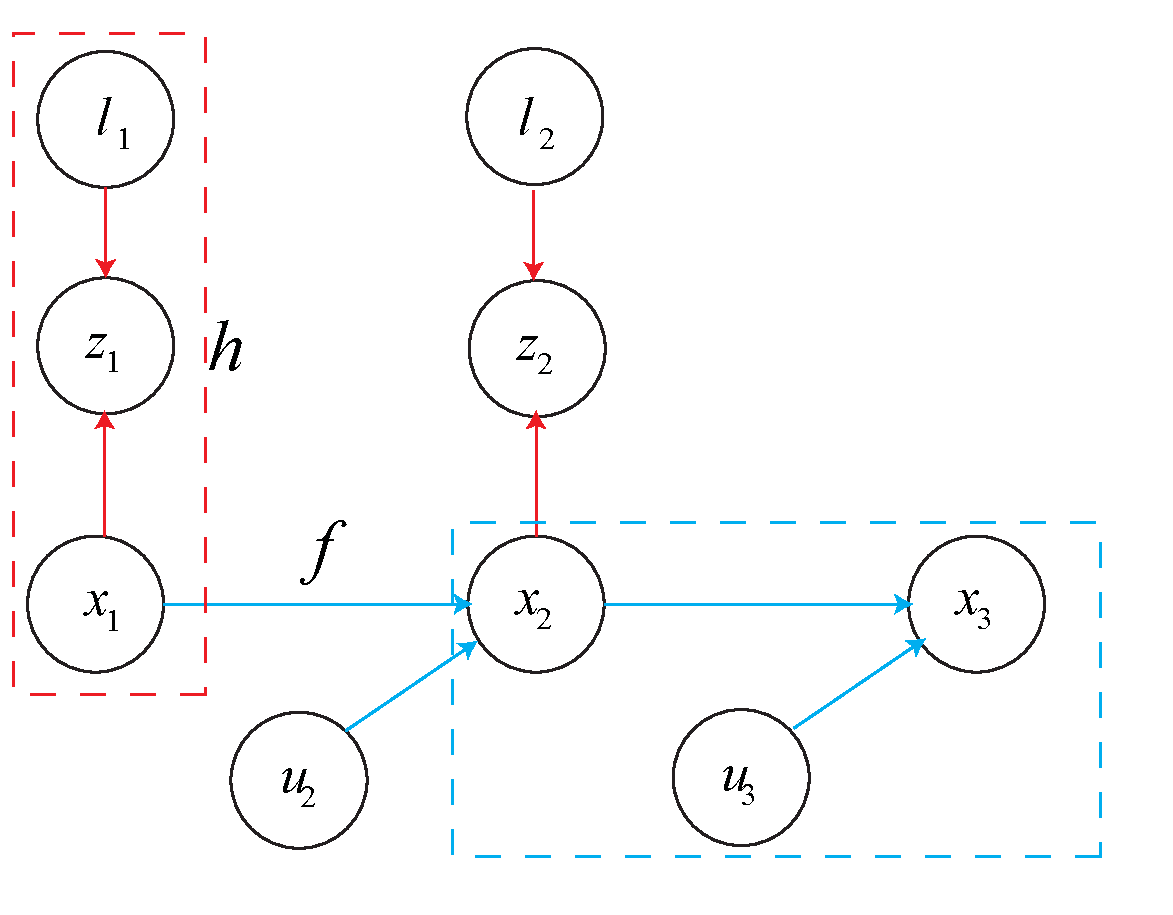
\includegraphics[width=0.54\textwidth]{backend2/bayes.pdf}
	\caption{以贝叶斯网络形式表达的SLAM过程示意图。竖线为运动方程,其他线为观测方程。虚线框表示一次观测,实线框表示一次运动。}
	\label{fig:bayes}
\end{figure}

\autoref{fig:bayes}~中的圆圈表示了贝叶斯网络的节点,也就是与图相关的随机变量,包括:
\begin{enumerate}
	\item 相机位姿形成的节点:$\bm{x}_1, \bm{x}_2 \cdots$。
	\item 输入量节点:$\bm{u}$。
	\item 路标节点:$\bm{l}$。
	\item 观测数据节点:$\bm{z}$。
\end{enumerate}

这组成了所有与SLAM过程相关的信息。另一方面,各线条表示了它们之间的关系,箭头表示\textbf{依赖关系}。例如,从$\bm{x}_1$指向$\bm{x}_2$的箭头,说明$\bm{x}_2$依赖于$\bm{x}_1$,此边表示的概率是$P(\bm{x}_2 | \bm{x}_1 )$——事实上,运动方程指出了从$\bm{x}_1$到$\bm{x}_2$的运动关系。我们观察实线框。这个框中,变量$\bm{x}_3$依赖于$\bm{x}_2, \bm{u}_3$。回忆运动方程:
\clearpage
\begin{equation}
\bm{x}_3 = f(\bm{x}_2, \bm{u}_3) + \bm{w}_3.
\end{equation}

它实际上给出了这几个变量的条件概率的度量:
\begin{equation}
P(\bm{x}_3 | \bm{x}_2, \bm{u}_3 ).
\end{equation}

同样,虚线框中的一次观测,亦说明观测方程给出了变量间的条件概率关系:
\begin{equation}
P(\bm{z}_1 | \bm{x}_1, \bm{l}_1 ).
\end{equation}

通过这种方式,我们构建了一个贝叶斯网络,它表达了所有变量,以及各个方程给出的变量之间的条件概率关系。请注意,这只是说贝叶斯网络\textbf{表达}了它们,还没有说到贝叶斯网络的求解。事实上,后端优化的目标,就是在这些既有的约束之上,通过调整贝叶斯网络中随机变量的取值,使整个后验概率达到最大:
\begin{equation}
\{ \bm{x}, \bm{l} \}^* = \arg \max \left( {{\bm{x}_0}} \right)\prod {P\left( {{\bm{x}_k}|{\bm{x}_{k - 1}},{\bm{u}_k}} \right)} \prod {P\left( {{\bm{z}_k}|{\bm{x}_i},{\bm{l}_j}} \right)} .
\end{equation}

直到现在为止,这和我们在图优化中谈论的东西并没有太大区别,我们只是把变量间的关系显式地用有向图给表达出来而已。这样一个由条件概率描述的贝叶斯网络,已经可以使用概率图模型中的算法进行求解了。不过,进一步观察,我们发现最大后验概率由许多项因子乘积而成,因此该贝叶斯网络又可以转化成一个\textbf{因子图(Factor Graph)}。

\subsection{因子图}
因子图是一种无向图,由两种节点组成:表示优化变量的\textbf{变量节点},以及表示因子的\textbf{因子节点}。如果我们把\autoref{fig:bayes}~表示成因子图,就可画成如\autoref{fig:factor}~所示的样子。

\begin{figure}[!htp]
	\centering
	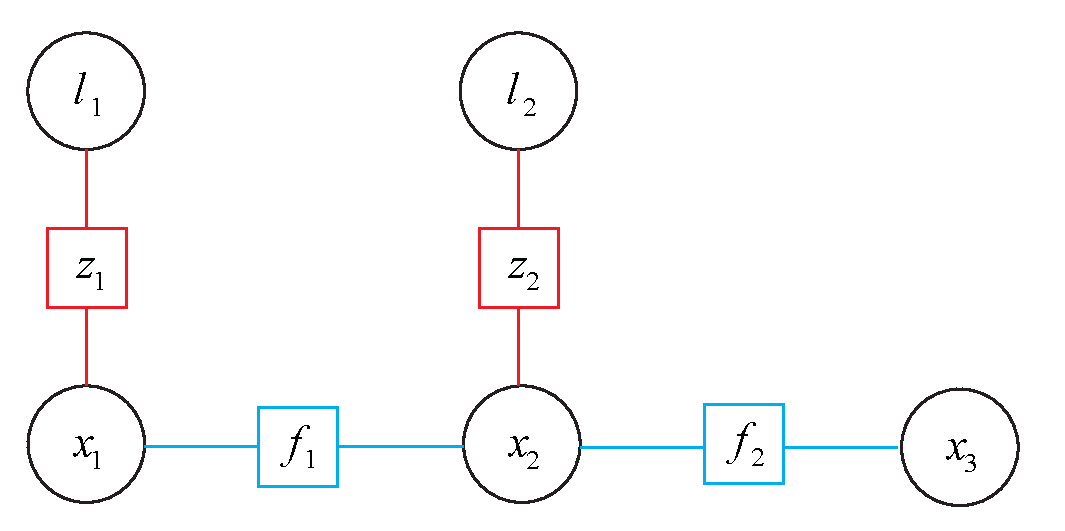
\includegraphics[width=0.6\textwidth]{backend2/factor.pdf}
	\caption{以因子图形式表达的SLAM过程示意图。圆圈为变量节点,方块为因子节点。}
	\label{fig:factor}
\end{figure}

在\autoref{fig:factor}~中,我们用圆圈表示变量节点。注意与贝叶斯网络不同,这里的变量是SLAM中待优化的部分,即相机位姿$\bm{x}$和路标$\bm{l}$,而没有观测$\bm{z}$和输入$\bm{u}$——因为这几个量是给定的而不是待优化的。与之相对,因子节点包含了待优化变量之间的关系,它们来自运动方程和观测方程。

对因子图的优化,就是调整各变量的值,使它们的因子之乘积最大化——它依然对应着一个优化问题。在通常的做法中,我们把各因子的条件概率取高斯分布的形式。考虑到运动方程为
\begin{equation}
{\bm{x}_k} = f\left( {{\bm{x}_{k - 1}},{\bm{u}_k}} \right) + {\bm{w}_k}.
\end{equation}

其中$\bm{w}_k \sim N(\bm{0}, \bm{R}_k)$。如果$\bm{x}_{k-1}$(实际上$\bm{x}_{k-1}$的取值还受其他因素影响)已知,那么:
\begin{equation}
P\left( {{\bm{x}_k}|{\bm{x}_{k - 1}}} \right) = N \left( {f\left( {{\bm{x}_{k - 1}},{\bm{u}_k}} \right),{\bm{R}_k}} \right).
\end{equation}

同理,对于观测数据,有:
\begin{equation}
P\left( {{\bm{z}_{kj}}|{\bm{x}_k},{\bm{l}_j}} \right) = N\left( {h\left( {{\bm{x}_k},{\bm{l}_j}} \right),{\bm{Q}_{kj}}} \right),
\end{equation}
其中$\bm{Q}_{kj}$为观测方程噪声项的协方差。

通过假设高斯分布,我们显式地表达了因子图优化的目标函数。和图优化一样,由于取最大的后验概率相当于取负对数的最小化,所以因子图优化也对应着一个和第6讲介绍的相似的最小二乘问题,我们可以用高斯牛顿法或列文伯格—马夸尔特方法求解一个因子图优化问题。类似于图优化,我们还可以使用单元的、二元的或多元的因子。这主要看它和几个变量节点有关。

\autoref{fig:factor-another}~是一个更实际的因子图的例子。

\begin{figure}[!htp]
	\centering
	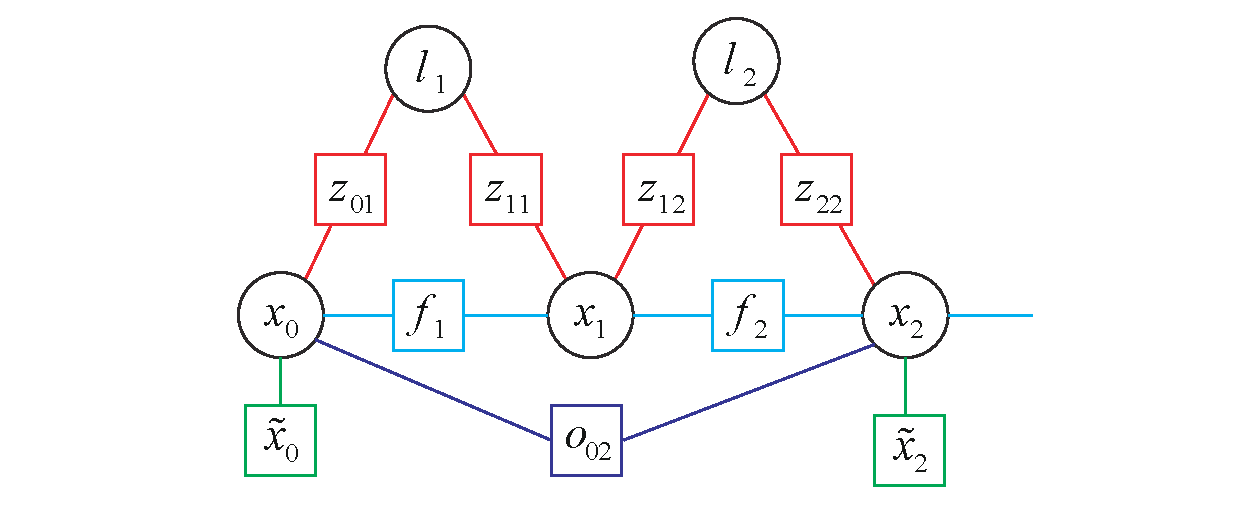
\includegraphics[width=0.75\textwidth]{backend2/factor-another.pdf}
	\caption{更加实际的因子图。添加了回环因子(底部中央)和先验因子(底部两侧)。}
	\label{fig:factor-another}
\end{figure}

运动方程和观测方程作为因子存在于图中。此外,我们可能对某些相机位姿具有先验信息——例如一辆在室外行驶的无人车,我们可能通过GPS信号确定了轨迹当中某些节点的位姿,那么就可以对这些位姿添加先验因子。因为可能表达成概率分布的信息有许多种,于是因子图也可以定义许多不同的因子,比如,轮式编码器的测量、IMU的测量,等等,使之成为一种非常通用的优化方式。

\subsection{增量特性}
然而,到现在为止,从优化角度来看,优化一个因子图和普通的图优化并没有太大的区别——因为我们最后面对的都是一个最小二乘问题,不断地寻找梯度,使目标函数下降。因子图优化的稀疏性也与图优化类似,我们可以通过稀疏QR分解、Schur补或Cholesky分解,加速对因子图优化的求解。所以我们不禁疑惑:因子图优化是否就是普通图优化换了种说法呢?事情并不完全是这样。

Kaess等人提出的iSAM(incremental Smooth and Mapping)\textsuperscript{\cite{Kaess2008}}中,对因子图进行了更加精细的处理,使得它可以\textbf{增量式}地处理后端优化。回忆第6讲的内容,我们知道,在普通的图优化中,最终要计算的是一个增量式方程。即如何调整目标函数
\begin{equation}
J (\bm{x}) = \sum\limits_k {\bm{e}_{v,k}^\mathrm{T} \bm{R}_k^{ - 1}{ \bm{e}_{v,k}}}  + \sum\limits_k {\sum\limits_j {\bm{e}_{y,k,j}^\mathrm{T} \bm{Q}_{k,j}^{ - 1}{\bm{e}_{y,k,j}}} }
\end{equation}
中的优化变量,使目标函数下降。无论采用哪种梯度下降策略,最后我们将碰到一个形如
\begin{equation}
\bm{H} \Delta \bm{x} = \bm{g}.
\end{equation}
的线性方程需要求解。上一讲,我们介绍了利用该方程中的稀疏性加速它的求解过程。然而,考虑到图优化并不是固定的,当机器人运动时,新的节点和边将被加入图中,使得它的规模不断增长。那么问题来了:是否每次新加一个节点,我们就要重新计算一遍所有节点的更新量呢?(包括雅可比的求取﹝或称线性化﹞和更新方程的计算。)

显然,这样做是不经济的,我们以\autoref{fig:incremental}~为例来解释增量更新的情况。这是一个位姿图。当我们按照里程计方式向其中添加节点时,受影响的节点可以近似地看成只有\textbf{最后一个与之相连的节点},而早先节点的估计值,可以近似地看成没有发生变化。因此就没有必要对它们进行优化。为什么要说近似呢?因为实际上新增节点还是会对之前的估计产生影响的,只是对最近的数据影响最大,对较远的数据影响很小,可以忽略掉。如果认为增量特性可行,那么这件事情可以为我们省掉大量的计算——至少我们不必在每次新增节点时,对\textbf{整个图}进行优化。不过,如果按照回环检测的方式添加节点,那么受影响的范围应该是回环开始到当前帧这一段中的所有节点,也就是整段轨迹都可能被重新调整。这虽然加大了计算量,然而我们依然无须优化整张图,因为回环之外的节点是不受影响的。综上所述,我们发现,在向图中添加节点时,通过分析受影响的区域,可以(直观上)减少一些没必要的计算,加速后端优化流程。

\begin{figure}[!htp]
	\centering
	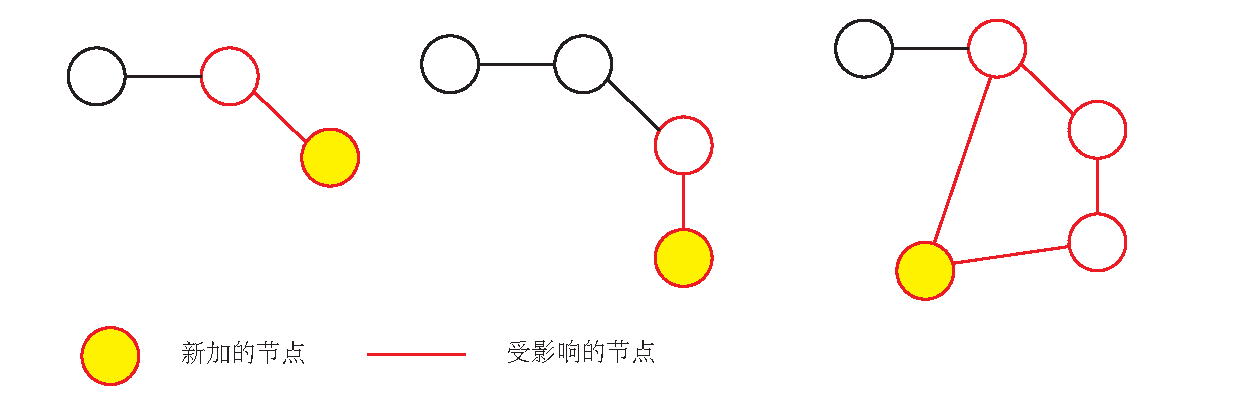
\includegraphics[width=0.72\textwidth]{backend2/incremental.pdf}
	\caption{增量更新示意图。}
	\label{fig:incremental}
\end{figure}

在此思想的基础上,Kaess等人提出的增量式因子图优化一定程度上解决了上面的问题。从技术层面上来看,我们希望在每次优化中保存一些中间结果;而当新的变量和因子加入时,首先分析它们因子图之间的连接和影响关系,考虑之前存储的信息有哪些可以继续利用,哪些必须重新计算,最后处理对增量的优化。话虽如此,由于具体的操作步骤需要介绍大量的技术细节,且牵涉到了概率图理论的知识,超出了本书的讨论范围。所以本节就作为可选阅读材料提供给读者。有兴趣的读者可以阅读iSAM、iSAM2等原始论文来了解它的细节处理。最后,尽管有增量分析,但我们必须清楚这里的受影响节点亦是近似的,所以在实际操作中,当图的规模发生一定程度的改变时,我们需要再做一次全图优化。

\section{\textsuperscript{\ttfamily *}实践:gtsam}
\subsection{安装gtsam 4.0}
下面,我们演示一个用因子图进行位姿图优化的例子。我们仍使用前面“球”的数据,不同的是,这次用因子图来优化它,而不是g2o中的位姿图。我们将使用Gtsam\textsuperscript{\cite{Dellaert2012}},它是一个基于因子图优化的SLAM后端库,理论来自文献\cite{Kaess2008, Kaess2011}。我们将在它的基础上,对上节“球”的例子进行优化。

gtsam最新版本为4.0,位于~\url{https://bitbucket.org/gtborg/gtsam}。你可以输入以下命令下载它:
\begin{lstlisting}
git clone https://bitbucket.org/gtborg/gtsam.git
\end{lstlisting}
由于gtsam比较大,我们没有在3rdparty文件夹中提供。与以往遇到的库一样,gtsam亦是一个cmake工程,我们按照cmake的方式来编译安装它。gtsam的依赖项比较少,主要是Eigen和tbb库。如果读者跟着本书一路走来,那么大多数库应该已经安装好了,只需安装tbb库即可:
\begin{lstlisting}
sudo apt-get install libtbb-dev
\end{lstlisting}

然后,使用cmake命令对gtsam进行编译安装,这里不再赘述。gtsam库比较大,集成了许多与因子图相关的内容,甚至底层的矩阵、李代数运算,所以编译安装会比较费时,请读者耐心等待。安装完成后,可以在/usr/local/include中找到头文件,在/usr/local/lib下找到库文件。gtsam的库文件比较简单,仅由一个libgtsam.so组成。所以你应该知道如何在自己的工程中书写CMakeLists.txt来调用gtsam了吧?

\subsection{位姿图优化}
下面我们来演示“球”的例子。与前面的实验一样,我们从sphere.g2o文件中读取节点和边的信息,转换为因子图交给gtsam处理,然后,把优化结果重新写到g2o文件,并“伪装”成g2o的节点和边以便显示。虽然这似乎没有体现出gtsam的“增量”特性,但至少我们可以通过这个例子体验一下它的用法。

\begin{lstlisting}[language=c++,caption=slambook/ch11/pose\_graph\_gtsam.cpp]
#include <iostream>
#include <fstream>
#include <string>
#include <Eigen/Core>

#include <sophus/se3.h>
#include <sophus/so3.h>

#include <gtsam/slam/dataset.h>
#include <gtsam/slam/BetweenFactor.h>
#include <gtsam/slam/PriorFactor.h>
#include <gtsam/nonlinear/GaussNewtonOptimizer.h>
#include <gtsam/nonlinear/LevenbergMarquardtOptimizer.h>

using namespace std;
using Sophus::SE3;
using Sophus::SO3;

/************************************************
* 本程序演示如何用 gtsam 进行位姿图优化
* sphere.g2o 是人工生成的一个 Pose graph, 我们来优化它。
* 与 g2o 相似,在 gtsam 中添加的是因子,相当于误差。
* **********************************************/

int main ( int argc, char** argv )
{
	if ( argc != 2 )
	{
		cout<<"Usage: pose_graph_gtsam sphere.g2o"<<endl;
		return 1;
	}
	ifstream fin ( argv[1] );
	if ( !fin )
	{
		cout<<"file "<<argv[1]<<" does not exist."<<endl;
		return 1;
	}
	
	gtsam::NonlinearFactorGraph::shared_ptr graph ( new gtsam::NonlinearFactorGraph );  // gtsam的因子图
	gtsam::Values::shared_ptr initial ( new gtsam::Values ); // 初始值
	// 从g2o文件中读取节点和边的信息
	int cntVertex=0, cntEdge = 0;
	cout<<"reading from g2o file"<<endl;
	
	while ( !fin.eof() )
	{
		string tag;
		fin>>tag;
		if ( tag == "VERTEX_SE3:QUAT" )
		{
			// 顶点
			gtsam::Key id;
			fin>>id;
			double data[7];
			for ( int i=0; i<7; i++ ) fin>>data[i];
			// 转换至gtsam的Pose3
			gtsam::Rot3 R = gtsam::Rot3::Quaternion ( data[6], data[3], data[4], data[5] );
			gtsam::Point3 t ( data[0], data[1], data[2] );
			initial->insert ( id, gtsam::Pose3 ( R,t ) );       // 添加初始值
			cntVertex++;
		}
		else if ( tag == "EDGE_SE3:QUAT" )
		{
			// 边,对应到因子图中的因子
			gtsam::Matrix m = gtsam::I_6x6;     // 信息矩阵
			gtsam::Key id1, id2;
			fin>>id1>>id2;
			double data[7];
			for ( int i=0; i<7; i++ ) fin>>data[i];
			gtsam::Rot3 R = gtsam::Rot3::Quaternion ( data[6], data[3], data[4], data[5] );
			gtsam::Point3 t ( data[0], data[1], data[2] );
			for ( int i=0; i<6; i++ )
				for ( int j=i; j<6; j++ )
				{
					double mij;
					fin>>mij;
					m ( i,j ) = mij;
					m ( j,i ) = mij;
				}
		
			// g2o 的信息矩阵定义方式与 gtsam 不同,这里对它进行修改
			gtsam::Matrix mgtsam = gtsam::I_6x6;
			mgtsam.block<3,3> ( 0,0 ) = m.block<3,3> ( 3,3 ); // cov rotation
			mgtsam.block<3,3> ( 3,3 ) = m.block<3,3> ( 0,0 ); // cov translation
			mgtsam.block<3,3> ( 0,3 ) = m.block<3,3> ( 0,3 ); // off diagonal
			mgtsam.block<3,3> ( 3,0 ) = m.block<3,3> ( 3,0 ); // off diagonal
			
			// 高斯噪声模型
			gtsam::SharedNoiseModel model = gtsam::noiseModel::Gaussian::Information ( mgtsam );        
			gtsam::NonlinearFactor::shared_ptr factor ( 
				new gtsam::BetweenFactor<gtsam::Pose3> ( id1, id2, gtsam::Pose3 ( R,t ), model ) // 添加一个因子
			);
			graph->push_back ( factor );
			cntEdge++;
		}
		if ( !fin.good() )
			break;
	}
	
	cout<<"read total "<<cntVertex<<" vertices, "<<cntEdge<<" edges."<<endl;
	// 固定第一个顶点,在 gtsam 中相当于添加一个先验因子 
	gtsam::NonlinearFactorGraph graphWithPrior = *graph;
	gtsam::noiseModel::Diagonal::shared_ptr priorModel = 
	gtsam::noiseModel::Diagonal::Variances (
		( gtsam::Vector ( 6 ) <<1e-6, 1e-6, 1e-6, 1e-6, 1e-6, 1e-6 ).finished() 
	);
	gtsam::Key firstKey = 0;
	for ( const gtsam::Values::ConstKeyValuePair& key_value: *initial )
	{
		cout<<"Adding prior to g2o file "<<endl;
		graphWithPrior.add ( gtsam::PriorFactor<gtsam::Pose3> ( 
			key_value.key, key_value.value.cast<gtsam::Pose3>(), priorModel ) 
		);
		break;
	}
	
	// 开始因子图优化,配置优化选项
	cout<<"optimizing the factor graph"<<endl;
	// 我们使用列文伯格—马夸尔特方法优化
	gtsam::LevenbergMarquardtParams params_lm;
	params_lm.setVerbosity("ERROR");
	params_lm.setMaxIterations(20);
	params_lm.setLinearSolverType("MULTIFRONTAL_QR");
	gtsam::LevenbergMarquardtOptimizer optimizer_LM( graphWithPrior, *initial, params_lm );
	
	// 你可以尝试下高斯牛顿法
	// gtsam::GaussNewtonParams params_gn;
	// params_gn.setVerbosity("ERROR");
	// params_gn.setMaxIterations(20);
	// params_gn.setLinearSolverType("MULTIFRONTAL_QR");
	// gtsam::GaussNewtonOptimizer optimizer ( graphWithPrior, *initial, params_gn );
	
	gtsam::Values result = optimizer_LM.optimize();
	cout<<"Optimization complete"<<endl;
	cout<<"initial error: "<<graph->error ( *initial ) <<endl;
	cout<<"final error: "<<graph->error ( result ) <<endl;
	
	cout<<"done. write to g2o ... "<<endl;
	// 写入 g2o 文件,同样伪装成 g2o 中的顶点和边,以便用 g2o_viewer 查看。
	// 顶点
	ofstream fout ( "result_gtsam.g2o" );
	for ( const gtsam::Values::ConstKeyValuePair& key_value: result )
	{
		gtsam::Pose3 pose = key_value.value.cast<gtsam::Pose3>();
		gtsam::Point3 p = pose.translation();
		gtsam::Quaternion q = pose.rotation().toQuaternion();
		fout<<"VERTEX_SE3:QUAT "<<key_value.key<<" "
		<<p.x() <<" "<<p.y() <<" "<<p.z() <<" "
		<<q.x()<<" "<<q.y()<<" "<<q.z()<<" "<<q.w()<<" "<<endl;
	}
	// 边 
	for ( gtsam::NonlinearFactor::shared_ptr factor: *graph )
	{
		gtsam::BetweenFactor<gtsam::Pose3>::shared_ptr f = dynamic_pointer_cast<gtsam::BetweenFactor<gtsam::Pose3>>( factor );
		if ( f )
		{
			gtsam::SharedNoiseModel model = f->noiseModel();
			gtsam::noiseModel::Gaussian::shared_ptr gaussianModel = dynamic_pointer_cast<gtsam::noiseModel::Gaussian>( model );
			if ( gaussianModel )
			{
				// write the edge information 
				gtsam::Matrix info = gaussianModel->R().transpose() * gaussianModel->R();
				gtsam::Pose3 pose = f->measured();
				gtsam::Point3 p = pose.translation();
				gtsam::Quaternion q = pose.rotation().toQuaternion();
				fout<<"EDGE_SE3:QUAT "<<f->key1()<<" "<<f->key2()<<" "
					<<p.x() <<" "<<p.y() <<" "<<p.z() <<" "
					<<q.x()<<" "<<q.y()<<" "<<q.z()<<" "<<q.w()<<" ";
				gtsam::Matrix infoG2o = gtsam::I_6x6;
				infoG2o.block(0,0,3,3) = info.block(3,3,3,3); // cov translation
				infoG2o.block(3,3,3,3) = info.block(0,0,3,3); // cov rotation
				infoG2o.block(0,3,3,3) = info.block(0,3,3,3); // off diagonal
				infoG2o.block(3,0,3,3) = info.block(3,0,3,3); // off diagonal
				for ( int i=0; i<6; i++ )
				for ( int j=i; j<6; j++ )
				{
					fout<<infoG2o(i,j)<<" ";
				}
				fout<<endl;
			}
		}
	}
	fout.close();
	cout<<"done."<<endl;
}
\end{lstlisting}

在演示程序中,我们以文本方式读取一个g2o文件,并完成了向gtsam接口的转换。请留意代码中g2o与gtsam的异同点。比如说相同的地方:

\begin{enumerate}
	\item 由于它们本质上都是同一个最小二乘优化问题,所以我们要设置的东西也是类似的。简而言之,即顶点(对应到因子图中的变量)的初值,以及边(对应到因子)的观测值,还有噪声大小。
	\item 在优化设置方面,同样可以使用高斯牛顿法或列文伯格—马夸尔特方法,并配置详细的参数,只不过接口略有不同。g2o通过构建优化算法对象来实现,而gtsam则是传入优化参数。
\end{enumerate}

不同的地方:
\begin{enumerate}
	\item g2o的噪声模型和gtsam稍有不同,我们在代码中做了一下转换。
	\item 在稀疏化的处理方面,gtsam可选择使用QR分解或Cholesky分解,尽管我们没有详细解释这方面的具体过程。读者可以追踪参数的配置方式,看看gtsam提供哪些求解方法。由于单纯的Pose Graph没有太多稀疏性可以利用,所以这里区别不大。
\end{enumerate}

最后,我们把gtsam的优化结果转换为g2o的输出文件,同样可以用g2o\_viewer查看此结果,如\autoref{fig:result-gtsam}~所示。

\begin{figure}[!ht]
	\centering
	\includegraphics[width=0.75\textwidth]{backend2/result-gtsam.pdf}
	\caption{gtsam的优化结果。}
	\label{fig:result-gtsam}
\end{figure}

下面是终端输出的优化信息:

\begin{lstlisting}
$ build/pose_graph_gtsam sphere.g2o 
reading from g2o file
read total 2500 vertices, 9799 edges.
Adding prior to g2o file 
optimizing the factor graph
Initial error: 4.7724e+09
newError: 6.07118e+08
errorThreshold: 6.07118e+08 > 0
absoluteDecrease: 4165284178.46 >= 1e-05
relativeDecrease: 0.872785675288 >= 1e-05
// 中间略
newError: 63793.9289983
errorThreshold: 63793.9289983 > 0
absoluteDecrease: 0.279685092828 >= 1e-05
relativeDecrease: 4.38417684928e-06 < 1e-05
converged
errorThreshold: 63793.9289983 <? 0
absoluteDecrease: 0.279685092828 <? 1e-05
relativeDecrease: 4.38417684928e-06 <? 1e-05
iterations: 5 >? 20
Optimization complete
initial error: 4772402087.24
final error: 63793.9289982
done. write to g2o ... 
done.
\end{lstlisting}

我们发现,虽然设置了最大迭代次数为20次,但gtsam只迭代了5次后算法就收敛了。同样,由于gtsam的误差定义方式与g2o不同,所以这里直接比较误差大小没有太大意义。如果用g2o\_viewer打开result\_gtsam.g2o文件并选择优化,就会发现在g2o度量下的误差大约为44360左右,和我们上一节使用李代数优化的结果一致,但gtsam的迭代次数更少一些。

有点遗憾的是,本例没有体现出gtsam的增量特性。如果我们把g2o文件中的节点和边按照时间排序,然后一个一个地放入gtsam中,可能对它的增量特征会有更好的表述。我们把这个实验留作习题,交给读者来完成。

\section*{习题}
\begin{enumerate}
	\item 如果将位姿图中的误差定义为$\Delta \bm{\xi}_{ij} = \bm{\xi}_i \circ \bm{\xi}_j^{-1}$,推导按照此定义的左乘扰动雅可比矩阵。
	\item 参照g2o的程序,在Ceres中实现对“球”位姿图的优化。
	\item 对“球”中的信息按照时间排序,分别喂给g2o和gtsam优化,比较它们的性能差异。
	\item[\optional] 阅读iSAM相关论文,理解它是如何实现增量式优化的。
\end{enumerate}
